\chapter{Method}\label{ch:Method}

\section{Data Collection}

The Reddit social media platform provides access to all comments posted on the platform through an easily accessible API. Acquiring a large dataset of comments was made simpler due to the existence of websites which regularly upload monthly comment datasets created using the Reddit API. The website used to download the dataset was \url{http://files.pushshift.io/reddit/comments/}. The Reddit comments within these datasets were stored in a single-line JSON format and the entire dataset was compressed with a Zstandard compression algorithm. Due to the large size of each monthly dataset, it was decided that only comments from December 2018 would be used as part of this research project. The dataset used was named RC\_2018-12.zst and was downloaded from the aforementioned website.

Despite only a single month of Reddit comments being chosen, the dataset was still too large to be analysed in any meaningful way. To further reduce the scope of the data it was decided to parse the original dataset into 10 smaller datasets, each consisting of a different subreddit. To ensure a good diversity of data, the 10 subreddits that were chosen belonged to thematically distinct Reddit communities. The subreddits used as part of the investigation are described in \autoref{tab:subredditDescriptions} below.

\begin{table}[H]
\centering
    \begin{tabular}{l|l}
        \bfseries Subreddit & \bfseries Description \\
        \hline
        the\_donald         & Donald Trump supporters            \\
        \hline
        politics            & Left wing American politics            \\
        \hline
        LateStageCapitalism & Anti-capitalism \\
        \hline
        dankmemes           & Humorous media and Meme culture          \\
        \hline
        GlobalOffensive     & Popular first-person shooter video game        \\
        \hline
        FortNiteBR          & Popular battle-royale video game           \\
        \hline
        funny               & ‘funny’ stories and images           \\
        \hline
        australia           & Australian news, politics, and nation-related posts            \\
        \hline
        canada              & Canadian news, politics, and nation-related posts                        \\
        \hline
        unitedkingdom       & United Kingdom news, politics, and nation-related posts \\
        \hline
    \end{tabular}
    \caption{\textit{Description of each Subreddit studied}}
    \label{tab:subredditDescriptions}
\end{table}

The first step was to split the original 140GB dataset into 1GB chunks of data. This was done to make the data easier to process. The subreddits were then parsed using a simple C++ program. C++ was chosen for the task due to its speed at completing parsing tasks on large files. The code of this parsing program can be seen in \autoref{ch:Appendix} \autoref{sec:AppendixParse}
 

\section {Data Exploration and Preparation}
\label{sec:DEP}
To carry out a cursory analysis of the data, the dataset containing all comments from the politics subreddit was loaded into RStudio using a package called jsonlite. The jsonlite package was used because of its ease of use and since it was benchmarked as one of the fastest json parsers. \cite{18} After the dataset was loaded, the dimensions of the data and the column names were probed as can be seen in \autoref{fig:codeImport} below.

\begin{figure}[H]
\begin{lstlisting}
> comments.all <- stream_in(file("politics.json"))
> nrow(comments.all)
[1] 1506774
> ncol(comments.all)
[1] 39
> colnames(comments.all)
 [1] "archived"                      "author"                        "author_created_utc"           
 [4] "author_flair_background_color" "author_flair_css_class"        "author_flair_richtext"        
 [7] "author_flair_template_id"      "author_flair_text"             "author_flair_text_color"      
[10] "author_flair_type"             "author_fullname"               "author_patreon_flair"         
[13] "body"                          "can_gild"                      "can_mod_post"                 
[16] "collapsed"                     "collapsed_reason"              "controversiality"             
[19] "created_utc"                   "distinguished"                 "edited"                       
[22] "gilded"                        "gildings"                      "id"                           
[25] "is_submitter"                  "link_id"                       "no_follow"                    
[28] "parent_id"                     "permalink"                     "removal_reason"               
[31] "retrieved_on"                  "score"                         "send_replies"                 
[34] "stickied"                      "subreddit"                     "subreddit_id"                 
[37] "subreddit_name_prefixed"       "subreddit_type"                "author_cakeday"     

\end{lstlisting}
\caption{\textit{Importing the data}}
\label{fig:codeImport}
\end{figure}

It immediately became apparent that the data featured a great deal of fields which were not going to be of value to the investigation, for example the fields regarding CSS styling. To further assist in the ability to analyse the data, these unnecessary fields were removed. \autoref{fig:selectColumns} reveals the columns  that were kept.

\begin{figure}[H]
\begin{lstlisting}
> colnames(comments.all)
[1] "author"             "author_created_utc" "body"               "created_utc"        "id"                
[6] "link_id"            "parent_id"          "permalink"          "score"         
\end{lstlisting}
\caption{\textit{Choosing relevant columns}}
\label{fig:selectColumns}
\end{figure}

As per the problem statement, this research will attempt to determine whether it is possible to predict the success of a comment. The success of a comment was defined by the score of the comment, as indicated by the score field within the dataset. Within this research, a comment was considered successful if it had a score greater than the average score of all comments within the subreddit. The method used to calculate the average score of comments within the politics subreddit is shown in \autoref{fig:avgScore} below.

\begin{figure}[H]
\begin{lstlisting}
> comments.all%>%summarize(Mean=mean(score))
     Mean
1 13.69  
\end{lstlisting}
\caption{\textit{Calculating average comment score}}
\label{fig:avgScore}
\end{figure}

As can be seen, any comment with a score above 13.69 within the politics subreddit would be considered successful. The above process was repeated for all other subreddits included within the investigation and the results are shown below in \autoref{tab:subredditSummaries}

\begin{table}
    \centering
    \begin{tabular}{c|c|c}
         \bfseries Subreddit & \bfseries Total Comments & \bfseries Average Score
         \csvreader[head to column names]{tableData/averagesandcounts.csv}{}
         {\\\hline\sub & \total & \avg}
    \end{tabular}
    \caption{\textit{Summary of each Subreddit studied}}
    \label{tab:subredditSummaries}
\end{table}

From the initial analysis, it is clear that the biggest Subreddit was /r/politics, which had 1856400 comments. The smallest Subreddit analysed was /r/LateStageCapitalism, which only had 42249 comments. Despite this fact, it boasted the highest average score out of all subreddits studied. 

From looking at the fields in the dataset it was clear that the content of the message, the length of the message, and the time of day, were going to be the most likely predictors of score. However, further study of the data revealed possible predictors that did not currently have fields associated with them. For example not all comments within the dataset are replying to a post, a significant amount of the comments are replying to other comments. How deep a comment is within a comment chain is highly likely to be a predictor of score. 

The tier which a comment existed on was determined using the id, link\_id, and parent\_id fields within the dataset. The link\_id field indicated which post the comment was associated with. If the parent\_id field was the same as the link\_id field it meant that the comment was at the top of the comment chain, which was then subsequently labelled as tier 1. Determining the tiers of other comments required following the parent ids of each comment until it reached the top of the chain. This was done by continuously left-joining the dataset with itself based on the parent\_id being equal to the link\_id. If a comment had a parent which was also within the dataset then the parent\_id of its parent comment was added as a new field in the dataset. A loop then iterated through the fields of each comment until the parent\_id was equal to the link\_id. The number of iterations required gave the comment tier. The code for this described process is shown in \autoref{ch:Appendix}: \autoref{sec:AppendexA1}

As well as this a field was added which indicated how long after the post was created that the comment was made. Since the dataset did not contain information on when the post was made, it was assumed that the earliest comment created within a post was when the post was created. After this, the created\_utc column was then converted from epoch time to a more recognisable time format which displayed the date and time of day. The code for this process is shown in \autoref{ch:Appendix}: \autoref{sec:AppendexA2}

The next step of data preparation involved correcting issues within the data values. Looking at the values within the data fields, two issues immediately became apparent. The first issue was that the dataset contained comments which had been deleted by a moderator or removed by the original author. On the Reddit platform, when a comment is deleted or removed it is not erased from view, it is instead replaced with the word [deleted] or [removed]. 

The second issue with the data was that it contained a large number of comments which had been authored by bots. Subreddits often use bots as automated moderators, and they frequently comment to inform other users that their comments had violated the rules. Since the bots post so frequently, it was easy to discover the names of the bot authors by counting the number of comments from each author and then sorting by top authors. The bots were then identified by a manual inspection of the top author names and the content of their comments. 

Both of these issues were corrected using the code displayed in \autoref{ch:Appendix} \autoref{sec:AppendexA3}


\section {Exploratory Text Analysis}
\label{sec:ETA}

Since the body of a comment was a likely predictor of score, an analysis of the words used in the comment, and the words used by the community as a whole, was required. To carry out text-mining techniques, the data had to first be subjected to several processing steps.

The first step was to sanitise the body of each comment. This involved converting all text to lowercase, and then removing all punctuation from the text. The next step was to tokenise the body of each comment into its constituent words. A token is described as a meaningful unit of text, such as a word \cite{21, 22}. Thus tokenisation involved taking each word within each comment and placing it in a new row of the dataset. The final step in pre-processing was to remove common English words in order to get a better idea of the words that are common to this particular community. A list of common English words can easily be accessed using the stop\_words variable within RStudio. The code for these pre-processing steps can be viewed in \autoref{ch:Appendix} \autoref{sec:AppendexA4}. The top 20 words from the politics subreddit are shown in \autoref{fig:politics_wordfreq} below.

\begin{figure}[H]
    \centering
    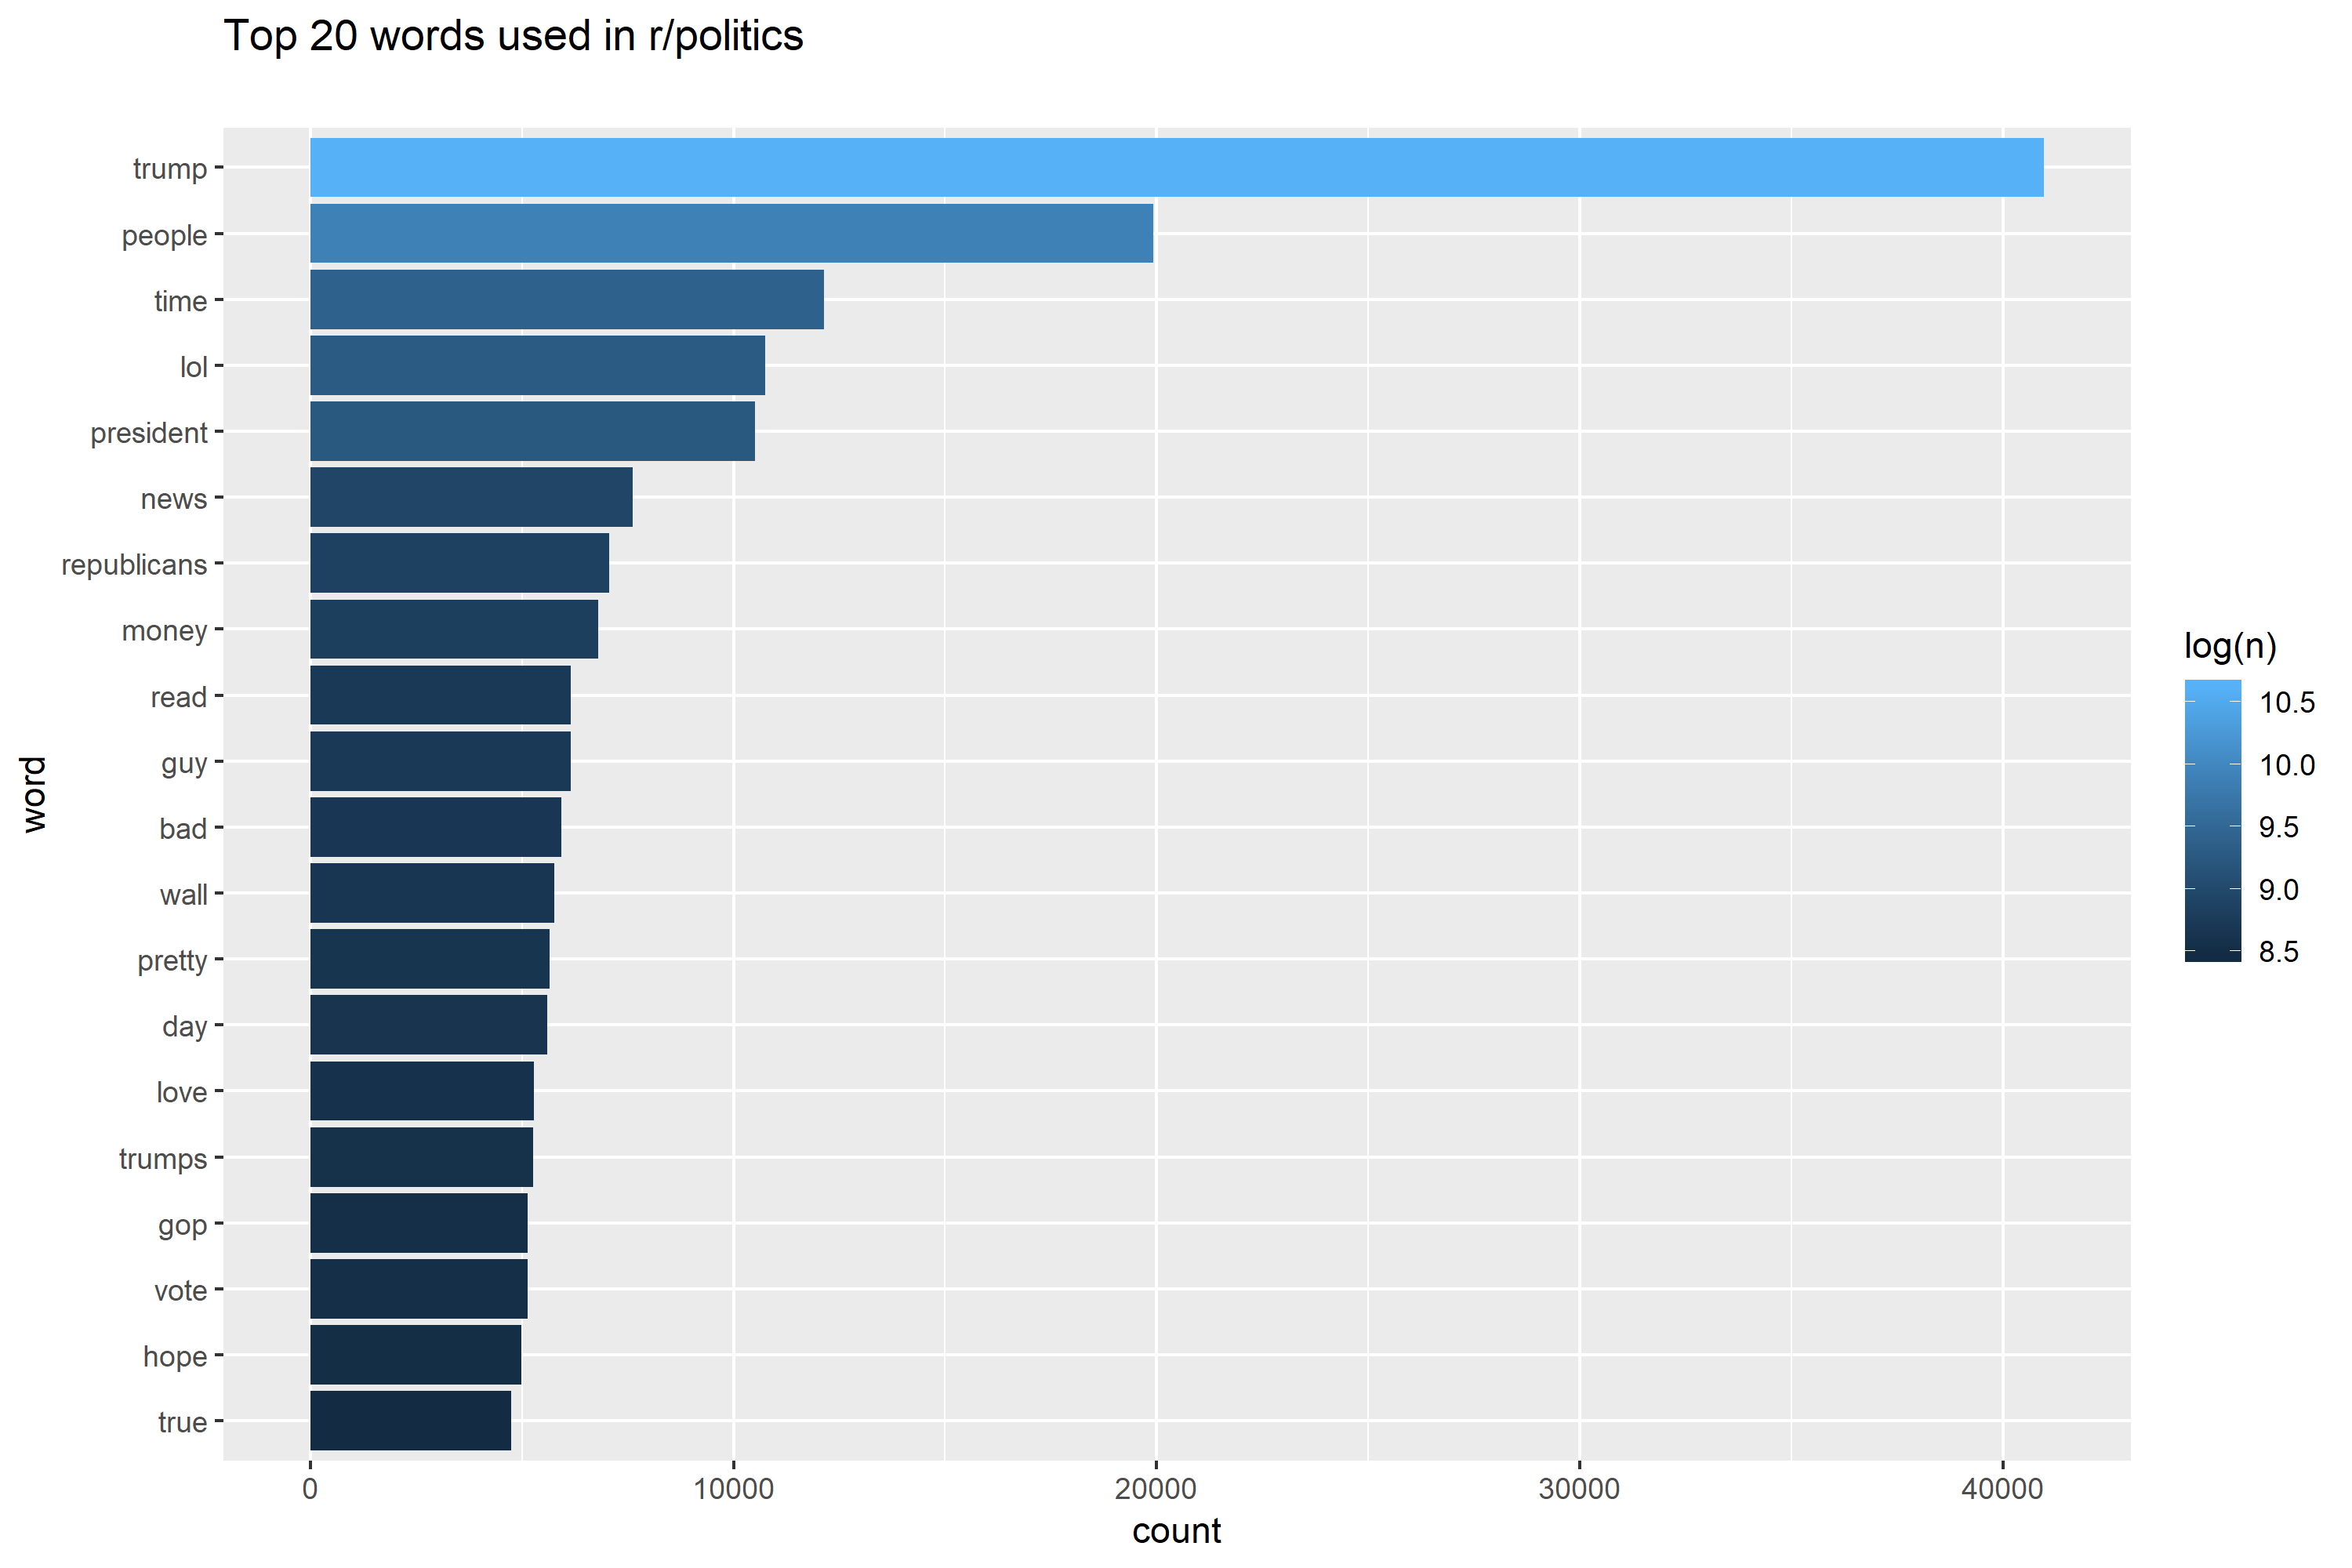
\includegraphics[width=1.0\textwidth]{graphs/politics_top_20.png}
    \caption{\textit{Most frequently used terms from r/politics. }}
    \label{fig:politics_wordfreq}
\end{figure}

As would be expected from a community surrounding american politcs, words like \textit{trump}, \textit{president}, and \textit{republicans} were frequently used. This list of words was saved, and the process repeated for all other subreddits studied. These community dictionaries would be useful in future classification efforts within individual communities.

See \autoref{ch:AppendixB} for additional graphs of word frequencies from other subreddits. Experiments were also initially done with bigrams, which are word pairs, and efforts were made to see how words are connected within a subreddit. Even though it was decided that bigrams and word connections would not be involved in later experiments, the graphs produced can be viewed in \autoref{ch:AppendixB} \autoref{sec:bigram}.


\section {Neural Network Classification}
\label{sec:neuralnet}
As part of this investigation, a neural network approach will by attempted. To create a neural network, an RStudio package called \textit{keras} was used. \textit{keras} is a simple yet powerful API allowing users to quickly create high-level neural networks. \cite{17} 

The neural network will take as an input a matrix of integers. Each row of the matrix will be a comment from the dataset, and each column of the matrix will contain an integer which maps to a word within the dictionary of common words created in \autoref{sec:ETA}.

The comments used for the neural network were an equally balanced set of successful and unsuccessful comments. The first step was to create a new dataset containing 20000 successful and 20000 unsuccessful comments. This determination was made using the average scores revealed in \autoref{sec:DEP}

Next, the words within each comment are separated into their own columns and converted to integers. This process was not done in RStudio and was instead carried out via a simple c++ program. This was done in C++ due to its speed of carrying out such tasks. The data was then read into a matrix within RStudio. The code for this C++ program is shown in \autoref{ch:Appendix} \autoref{sec:AppendexA5}

The next step was to define the neural network which would be used. After multiple trial and error attempts, it was finally decided to use the following model shown below in \autoref{fig:KerasModel}

\begin{figure}[H]
\begin{lstlisting}
#Configure the model
vocab_size <- 15001
model <- keras_model_sequential()
model %>% 
  layer_embedding(input_dim = vocab_size, output_dim = 128)%>%
  layer_global_average_pooling_1d()%>%
  layer_dropout(0.8)%>%
  layer_dense(units = 128, activation = "relu")%>%
  layer_dropout(0.8)%>%
  layer_dense(units = 128, activation = "relu")%>%
  layer_dropout(0.8)%>%
  layer_dense(units = 1, activation = "sigmoid")

model %>% summary()

#ADD LOSS FUNCTION AND OPTIMIZER
model %>% compile(
  optimizer = 'adam',
  loss = 'binary_crossentropy',
  metrics = 'accuracy'
)
\end{lstlisting}
\caption{\textit{The Neural Network}}
\label{fig:KerasModel}
\end{figure}

The model used as part of the network consists of an input layer of size 15000. This layer essentially consists of 15000 inputs which can have a value of 0 or 1. These inputs refer to the aforementioned integer matrix of comments. The model then also features 2 hidden layers containing 128 neurons each and ends with a layer with a single neuron which acts as a binary classifier. The model is also interspersed with dropout layers in order to help prevent over-fitting of the training data set.

The optimiser and loss functions were chosen due to their suitability for binary-classification in neural-networks. \cite{19, 20}

The comment dataset that was previously created was then randomised and split into training, validation, and testing sets with a ratio of 17:2:1. The model was then trained over 20 epochs and the accuracy and fit of the model was evaluated.

The results of this model can be viewed at \autoref{ch:Results} \autoref{sec:NNclass}, and the entire code can be found at \autoref{ch:Appendix} \autoref{sec:AppendexNeural}.


